\subsection{Достатні умови збіжності}

\begin{definition}
    $x_0 \in D_f$ називається \textit{регулярною точкою функції} $f: \RR \to \RR$ якщо функція має скінченні односторонні похідні:
    \begin{equation}
        \exists f (x_0 \pm 0) \in \RR
    \end{equation}
    і
    \begin{equation}
        f(x_0) = \frac{f(x_0 + 0) + f(x_0 - 0)}{2}.
    \end{equation}
\end{definition}

\begin{definition}
    Кажуть, що функція $f$ задовольняє у точці $x_0$ \textit{умову Діні}, якщо $\exists h > 0$ таке, що обидва невласні інтеграли другого роду
    \begin{equation}
        \int_0^h \frac{|f(x_0 \pm t) - f(x_0 \pm 0)|}{t} \diff t
    \end{equation}
    є збіжними.
\end{definition}

\begin{theorem}[ознака Діні збіжності тригонометричного ряду Фур'є]
    Якщо $f \in R([-\pi, \pi])$ --- $2\pi$-періодична і задовольняє у регулярній точці $x_0$ умову Діні, то тригонометричний ряд Фур'є функції $f$ у точці $x_0$ збігається до $f(x_0)$.
\end{theorem}
\begin{proof}
    Нам необхідно показати, що послідовність часткових сум $S_n(x_0) \to f(x_0)$. З одного боку, можна записати, що
    \begin{equation}
        S_n(x_0) = \frac{1}{\pi} \int_0^\pi (f(x_0 + t) + f(x_0 - t)) D_n(t) \diff t,
    \end{equation}
    а з іншого
    \begin{equation}
        \begin{aligned}
            f(x_0)
            &= \frac{2}{\pi} \int_0^\pi \frac{f(x_0 + 0) + f(x_0 - 0)}{2} D_n(t) \diff t = \\
            &= \frac{1}{\pi} \int_0^\pi (f(x_0 + 0) + f(x_0 - 0)) D_n(t) \diff t.
        \end{aligned}
    \end{equation}
    
    Розглянемо тепер різницю
    \begin{equation}
        \begin{aligned}
            S_n(x_0) - f(x_0)
            &= \frac{1}{\pi} \int_0^\pi (f(x_0 + t) - f(x_0 + 0)) D_n(t) \diff t + \\
            &\quad + \frac{1}{\pi} \int_0^\pi (f(x_0 - t) - f(x_0 - 0)) D_n(t) \diff t.
        \end{aligned}
    \end{equation}
    
    Нагадаємо, що ми хочемо показати, що вираз вище $\xrightarrow[n \to \infty]{} 0$. \medskip
    
    З умови Діні можна записати
    \begin{equation}
        \forall \epsilon > 0 \exists \delta \in (0, h): \quad \int_0^\delta \frac{|f(x_0 + t) - f(x_0 + 0)|}{t} \diff t < \epsilon.
    \end{equation}
    
    А тоді можемо розбити кожний з двох попередніх інтегралів на дві частини і оцінити кожну окремо. Проробимо ці дії для інтегралу з $f(x_0 + t) - f(x_0 + 0)$, для другого все буде аналогічно:
    \begin{multline}
        \int_0^\pi (f(x_0 + t) - f(x_0 + 0)) D_n(t) \diff t = \int_0^\delta (f(x_0 + t) - f(x_0 + 0)) D_n(t) \diff t + \\
        + \int_\delta^\pi (f(x_0 + t) - f(x_0 + 0)) D_n(t) \diff t = A_n(\delta) + \beta_n(\delta).
    \end{multline}
    
    Оцінимо $|A_n(x_0)|$:
    \begin{equation}
        \begin{aligned}
            |A_n(x_0)|
            &\le \int_0^\delta |f(x_0 + t) - f(x_0 + 0)| |D_n(t)| \diff t \le \\
            &\le \frac{\pi}{2} \int_0^\delta \frac{|f(x_0 + t) - f(x_0 + 0)|}{|t|} \diff t < \frac{\pi \epsilon}{2}.
        \end{aligned}
    \end{equation}
    
    Оцінимо $|\beta_n(x_0)|$:
    \begin{equation}
        \begin{aligned}
            |\beta_n(x_0)|
            &= \int_\delta^\pi \frac{f(x_0 + t) - f(x_0 + 0)}{2 \sin \tfrac{t}{2}} \sin (n + \tfrac{1}{2}) t \diff t \xrightarrow[n \to \infty]{} 0,
        \end{aligned}
    \end{equation}
    за однією із доведених властивостей ядра Діріхле.
\end{proof}

\subsection{Умова і ознака збіжності Гьольдера}

\begin{definition}
    Кажуть, що $f: \RR \to \RR$ у точці $x_0$ задовольняє умову Гьольдера (H\"older) порядку $\alpha$ зі сталою $m$ якщо $\exists \delta > 0$: $\forall t \in (0, \delta)$:
    \begin{equation}
        |f(x_0 \pm t) - f(x_0 \pm 0)| \le m \cdot t^\alpha. 
    \end{equation}
\end{definition}

\begin{theorem}[ознака Гьольдера збіжності тригонометрчиного ряду Фур'є]
    Якщо $f \in R([-\pi, \pi])$ --- $2\pi$-періодична і задовольняє у регулярній точці $x_0$ умову Гьольдера з $\alpha > 0$, то ряд Фур'є функції $f$ у точці $x_0$ зігається до $f(x_0)$.
\end{theorem}
\begin{proof}
    З умови Гьольдера одразу отримуємо
    \begin{equation}
        \left| \frac{f(x_0 \pm t) - f(x_0 \pm 0)}{t} \right| \le \frac{m \cdot t^\alpha}{t} = \frac{m}{t^{1 - \alpha}}.
    \end{equation}
    
    Але $1 - \alpha < 1$, і тому інтеграл з умови Діні збіжний, тобто можна скористатися ознакою Діні.
\end{proof}

\begin{corollary}
    Якщо $x_0$ --- точка розриву першого роду функції $f$ і $f$ задовольняє умову Гьольдера в $x_0$, то її ряд Фур'є у цій точці збігається до
    \begin{equation}
        \frac{f(x_0 + 0) - f(x_0 - 0)}{2}.
    \end{equation}
\end{corollary}

Будемо позначати
\begin{equation}
    f_\pm'(x_0 \pm 0) = \lim_{t \downarrow 0} \frac{f(x_0 \pm t) - f(x_0 \pm 0)}{t}.
\end{equation}

\begin{theorem}[ознака збіжності ряду Фур'є функції з узагальненими односторонніми похідними]
    Нехай $f \in R([-\pi, \pi])$ --- $2\pi$-періодична, і має скінченні узагальнені односторонні похідні, тоді
    \begin{enumerate}
        \item якщо $x_0$ --- регулярна, то ряд Фур'є збінається до $\frac{f(x_0 + 0) - f(x_0 - 0)}{2}$;
        \item якщо $\exists f'(x_0)$ то ряд Фур'є збігається до $f(x_0)$.
    \end{enumerate}
\end{theorem}
\begin{proof}
    Зі скінченності узагальнених односторонніх похідних маємо
    \begin{equation}
        \exists \delta > 0: \forall t \in (0, \delta) \quad \frac{|f(x_0 \pm t) - f(x_0 \pm 0)|}{t} \le m.
    \end{equation}
    
    А далі з ознаки Гьольдера випливає збіжність.
\end{proof}

\begin{theorem}[ознака збіжності ряду Фур'є кусково-гладкої функції]
    Якщо $f$ --- кусково-гладка на $[-\pi,\pi]$, $2\pi$-періодична функція, то її ряд Фур'є у точці $x_0$ збігається до 
    \begin{enumerate}
        \item $f(x_0)$ якщо $f$ неперервна в $x_0$;
        \item $\frac{f(x_0 + 0) + f(x_0 - 0)}{2}$ якщо $f$ має розрив першого роду у точці $x_0$.
    \end{enumerate}
\end{theorem}

Нехай $f$ --- $2T$-періодична. Тоді можна записати
\begin{equation}
    \frac{a_0}{2} + \sum \left( a_n \cos \frac{n \pi x}{T} + b_n \sin \frac{n \pi x}{T} \right),
\end{equation}
де
\begin{equation}
    a_n = \frac{1}{T} \int_{-T}^T f(x) \cos \frac{n \pi x}{T} \diff x.
\end{equation}

Причому, якщо $f$ --- парна, то $b_n = 0$, а
\begin{equation}
    a_n = \frac{2}{T} \int_0^T f(x) \cos \frac{n \pi x}{T} \diff x.
\end{equation}

\begin{example}
    $f(x) = x$ розвинути в ряд Фур'є на $(0, 1)$ по:
    \begin{enumerate}
        \item $\sin$;
        \item $\cos$;
        \item $\sin, \cos$.
    \end{enumerate}
    
    У всіх пунктах намалювати графік суми ряду Фур'є, який вийде.
\end{example}
\begin{solution}
    $2T$-періодично продовжуємо на $[-1,1]$ непарним чином, тоді $b_n = \ldots = \frac{2 (-1)^{n + 1}}{\pi n}$.

    \begin{figure}[H]
        \centering
        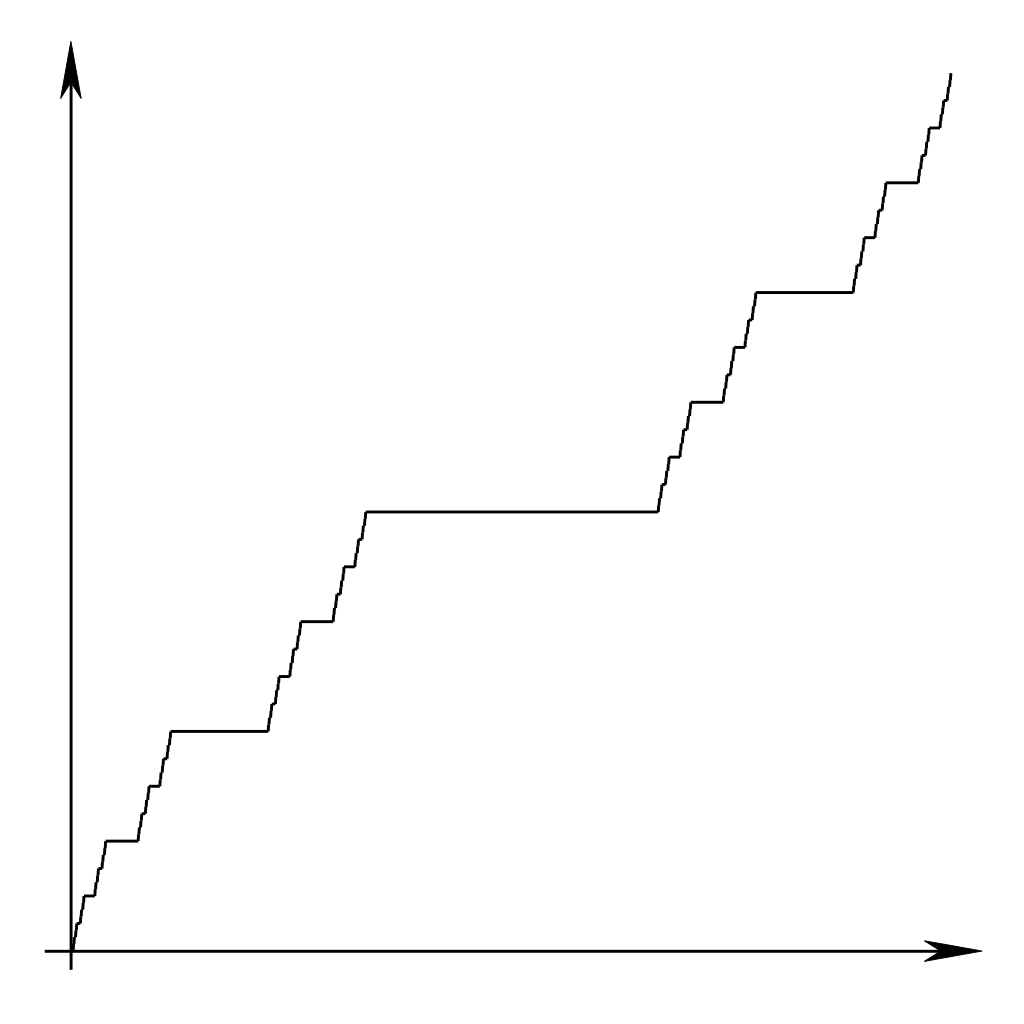
\includegraphics{03.png}
        \caption{Графік суми ряду Фур'є такий же як і початкової функції, що ілюструє істинність попередньої теореми}
    \end{figure}
\end{solution}
